\chapter{Planificación}

\section{Fases}

Las fases seguidas a lo largo del desarrollo de este proyecto son las que se detallan a continuación:

\begin{itemize}
	\item \textbf{Fase 1:} Espeficiación del proyecto. Se establecen los objetivos a cumplir para que el proyecto se considere completado.
	\item \textbf{Fase 2:} Planificación. Se definen las fases de desarrollo del sistema y las actividades a desarrollar en cada una de ellas.
	\item \textbf{Fase 3:} Análisis. Se realiza el análisis de requisitos del sistema. 
	\item \textbf{Fase 4:} Adquisición del conocimiento. Se obtienen los conocimientos necesarios para poder crear el sistema experto.
	\item \textbf{Fase 5:} Diseño. Se analizan todos los aspectos del proyecto para concretar su desarrollo.
	\item \textbf{Fase 6:} Implementación. Se procede a implementar todas las funcionalidades necesarias.
	\item \textbf{Fase 7:} Pruebas y validación. Se verifica y valida el sistema para comprobar su correcto funcionamiento.
	\item \textbf{Fase 8:} Documentación. Se realiza toda la documentación informativa y explicativa.
\end{itemize}


\section{Lista de tareas}

\begin{itemize}
	\item \textbf{Especificación del proyecto:}
	\begin{itemize}
		\item Determinación de objetivos.
		\item Determinación de requisitos.
	\end{itemize}
\end{itemize}

\bigskip

\begin{itemize}
	\item \textbf{Planificación:}
	\begin{itemize}
		\item Lista de actividades.
		\item Recursos humanos.
		\item Temporización.
	\end{itemize}
\end{itemize}

\bigskip

\begin{itemize}
	\item \textbf{Análisis:}
	\begin{itemize}
		\item Análisis de requisitos.
		\item Descripción de casos de uso.
		\item Diagramas de casos de uso.
		\item Diagramas de actividad.
	\end{itemize}
\end{itemize}

\bigskip

\begin{itemize}
	\item \textbf{Adquisición del conocimiento:}
	\begin{itemize}
		\item Extracción de conocimientos.
		\item Educción de conocimientos.
		\item Estructuración de conocimientos.
	\end{itemize}
\end{itemize}

\bigskip

\begin{itemize}
	\item \textbf{Diseño:}
	\begin{itemize}
		\item Selección de herramientas.
		\item Diseño de la arquitectura.
	\end{itemize}
\end{itemize}

\bigskip

\begin{itemize}
	\item \textbf{Implementación:}
	\begin{itemize}
		\item Implementación del sistema experto.
		\item Implementación de la interfaz.
	\end{itemize}
\end{itemize}

\bigskip

\begin{itemize}
	\item \textbf{Pruebas y validación:}
	\begin{itemize}
		\item Verificación.
		\item Validación del sistema por un experto.
	\end{itemize}
\end{itemize}

\bigskip

\begin{itemize}
	\item \textbf{Documentación:}
	\begin{itemize}
		\item Documentación del proyecto.
	\end{itemize}
\end{itemize}

\section{Recursos humanos}

Para poder desarrollar este proyecto he contado con la ayuda de varios músicos y compositores profesionales que me han ayudado a crear la base de conocimiento del sistema. Además, también he contado con profesores del Conservatorio Profesional de Música Ángel Barrios de Granada para poder llevar a cabo su validación.

Los expertos consultados han sido:

\begin{itemize}
	\item Alberto José Moreno Montes (Violista y compositor)
	\item Isabel Salado Ortega (Pianista)
	\item Clara Luz Fernández Vecino (Profesora de armonía)
\end{itemize}

\section{Temporización}

Para percibir de forma más visual la planificación temporal se la figuras \ref{fig1.4.1}, \ref{fig1.4.2} y \ref{fig1.4.3}.

\begin{figure}[H]
	\centering
	\hspace*{-1.2in}
	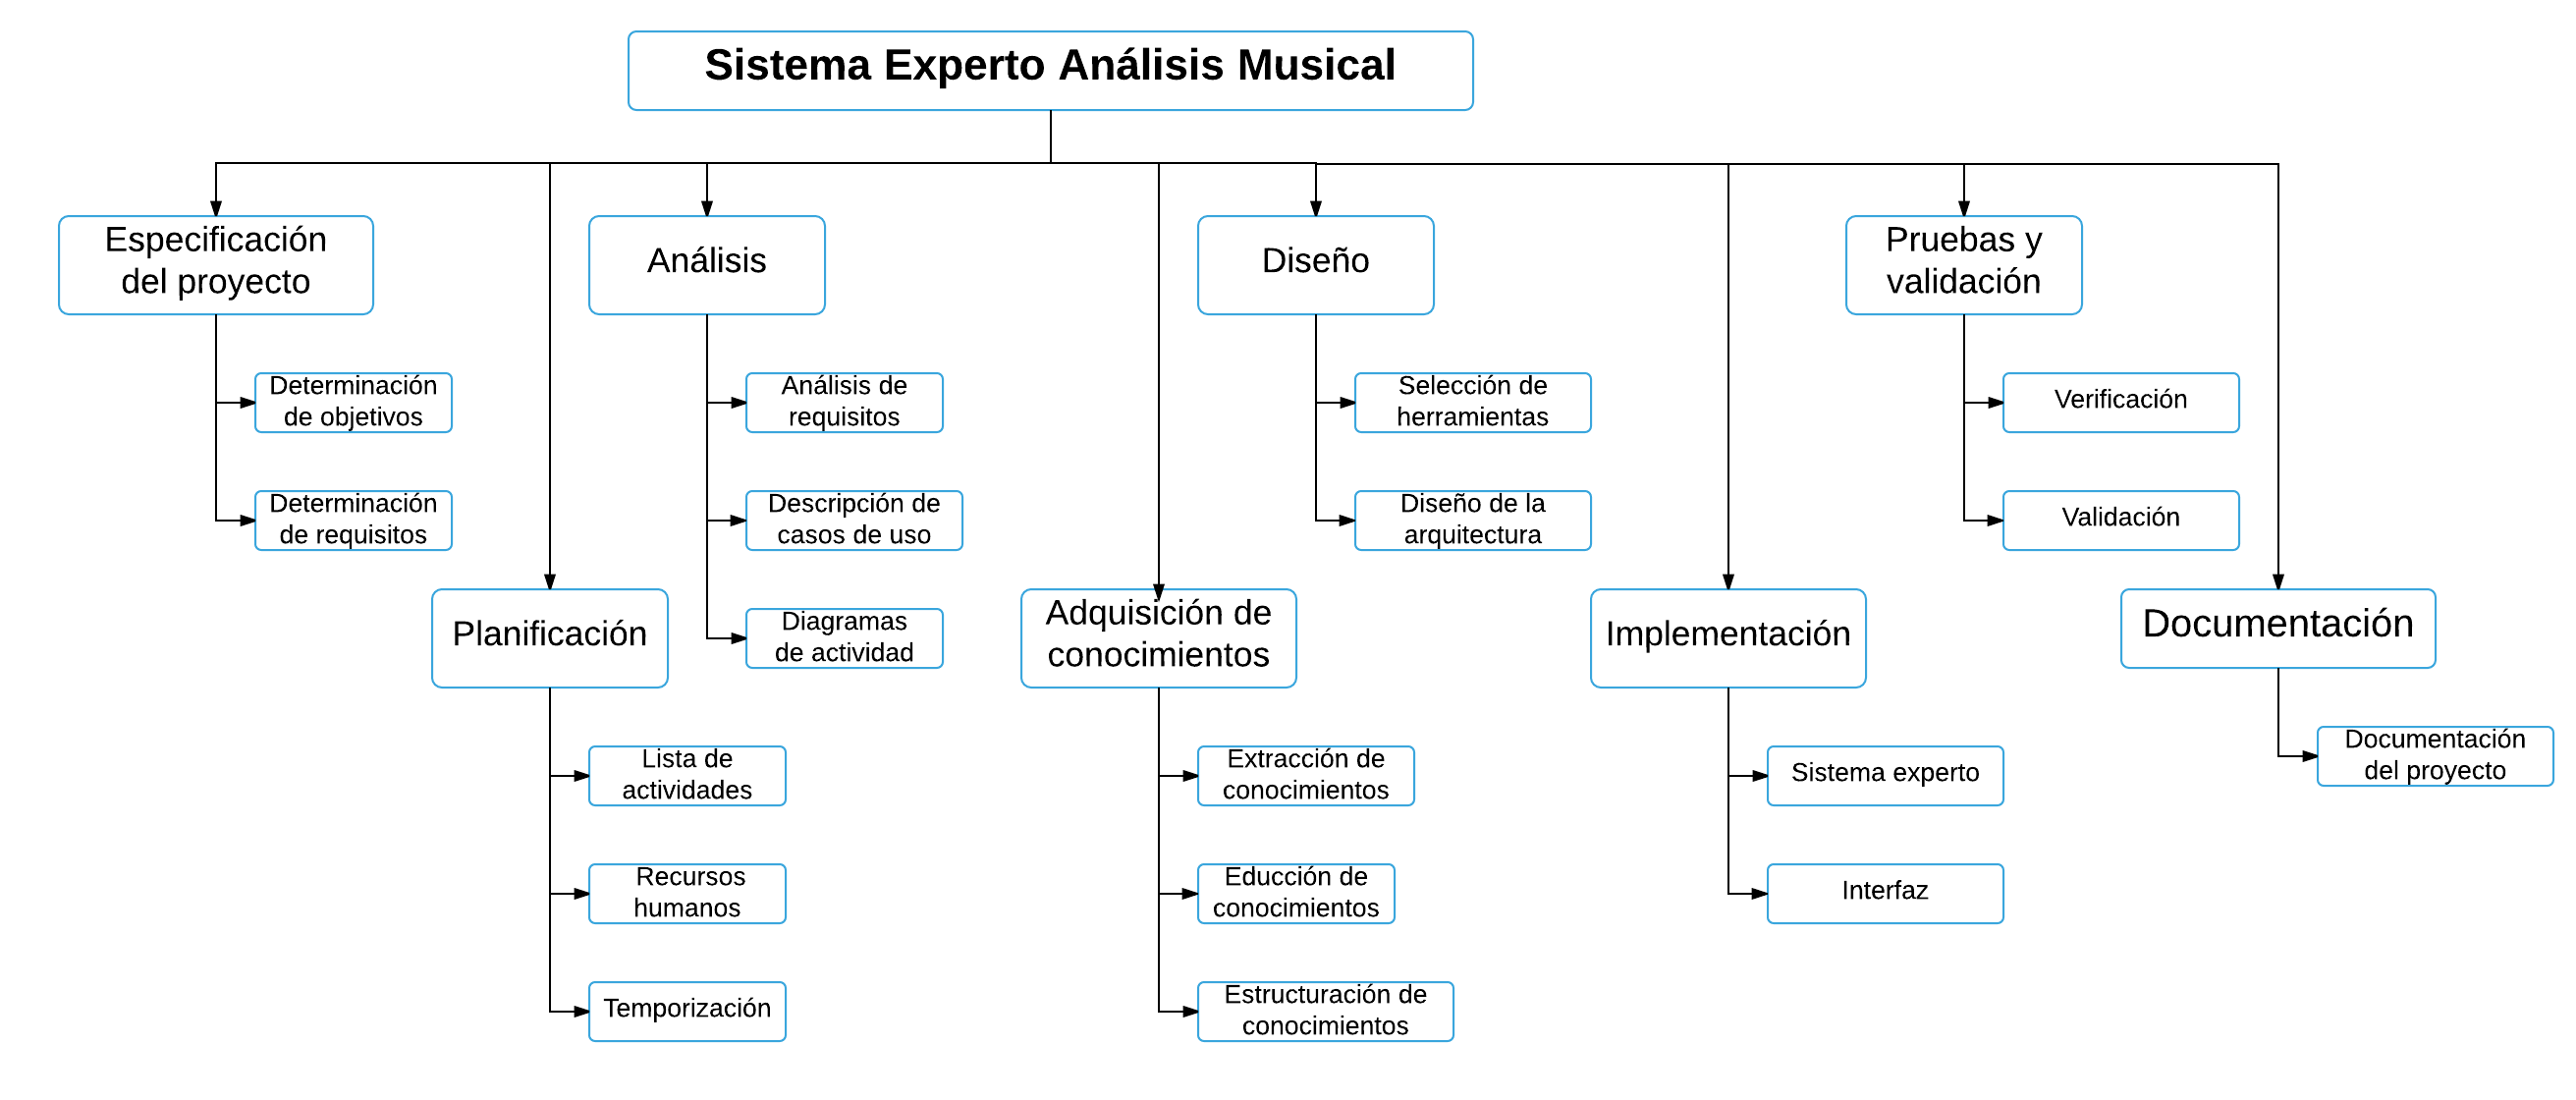
\includegraphics[scale=0.5]{imagenes/diagrama_edt.png}
	\caption{Diagrama de estructura de descomposición de trabajo}
	\label{fig1.4.1}
\end{figure}

\begin{figure}[H]
	\centering
	\hspace*{-0.6in}
	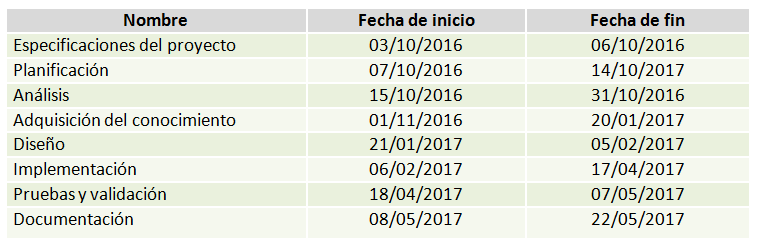
\includegraphics[scale=0.7]{imagenes/diagrama_tareas.png}
	\caption{Temporización de las tareas}
	\label{fig1.4.2}
\end{figure}

\bigskip
\bigskip

\begin{figure}[H]
	\centering
	\hspace*{-0.6in}
	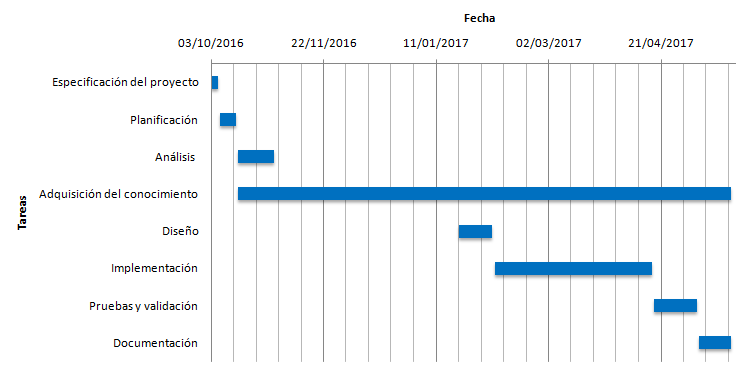
\includegraphics[scale=0.80]{imagenes/diagrama_gantt.png}
	\caption{Diagrama de Gantt}
	\label{fig1.4.3}
\end{figure}